\section{Single-Day Validation}
\label{sec:single_day}

\subsection{Data and Experimental Setup}

We analyze S\&P 500 ETF (SPY) options data covering 242 trading days in 2024 (95.6\% of trading days), with end-of-day snapshots including complete bid/ask spreads, open interest, implied volatility, and Greeks for all available strikes. All 242 days exhibited negative net gamma exposure (GEX $< -$\$2B), reflecting the persistent 0DTE-driven regime. We employ two prompt templates: an \textit{unbiased} template providing only raw GEX values without classification hints, and a \textit{biased} template including regime labels to establish detection ceiling.

The single-day validation uses OpenAI's o3-mini and o4-mini reasoning models, processing batches of pattern tests at $\sim$\$0.01 per validation across 726 total tests (242 days $\times$ 3 patterns).

\subsection{Detection Results}

Table~\ref{tab:detection} presents detection rates across all three dealer constraint patterns. The unbiased configuration achieves 71.5\% average detection (95\% CI: 68.2\%--74.8\%), significantly exceeding the 60\% threshold ($p < 0.001$). All patterns achieve 100\% detection with biased prompts, quantifying the 28.5pp impact of leading information.

\begin{table}[!htbp]
\centering
\caption{Pattern Detection Rates and Accuracy (242 Trading Days)}
\label{tab:detection}
\small
\begin{tabular}{@{}lcccc@{}}
\toprule
\textbf{Pattern} & \multicolumn{2}{c}{\textbf{Detection Rate}} & \textbf{Accuracy} \\
 & Unbiased & Biased & \\
\midrule
Gamma Positioning & 69.4\% & 100\% & 92.5\% \\
Stock Pinning & 67.4\% & 100\% & 90.4\% \\
0DTE Hedging & 77.7\% & 100\% & 90.8\% \\
\midrule
\textbf{Average} & \textbf{71.5\%} & \textbf{100\%} & \textbf{90.9\%} \\
\bottomrule
\end{tabular}
\end{table}

Of 726 total pattern tests, 519 detections yielded 472 materialized predictions (90.9\% pooled accuracy). Power analysis confirms $>$99\% power for detecting the observed rate versus a 50\% random baseline.

\subsection{Raw Chain Validation}
\label{subsec:raw_chain}

A critical methodological question: does the LLM genuinely identify structural constraints, or merely pattern-match on pre-calculated GEX? We conduct a \textbf{raw chain validation} providing \textit{only} strike-by-strike options data---open interest, implied volatility, volume, and bid-ask spreads---with no derived metrics. Temporal obfuscation remains identical.

\begin{table}[!htbp]
\centering
\caption{Detection: Raw Chain vs.\ GEX-Assisted Baseline ($n = 13$)}
\label{tab:raw_chain}
\begin{tabular}{@{}lcc@{}}
\toprule
\textbf{Method} & \textbf{Detection Rate} & \textbf{Avg Confidence} \\
\midrule
Raw Chain (no GEX) & 92.3\% (12/13) & 71.2 \\
Baseline (with GEX) & 61.5\% (8/13) & 77.5 \\
\midrule
\textbf{Difference} & \textbf{+30.8pp} & $-$6.3 \\
\bottomrule
\end{tabular}
\end{table}

Fig.~\ref{fig:raw_chain} visualizes this comparison. The raw chain method \textit{outperforms} the GEX-assisted baseline by 30.8pp, directly refuting the pattern-matching critique. When we remove the ``\$-32B GEX'' label entirely, detection \textit{improves}.

\begin{figure}[!htbp]
\centering
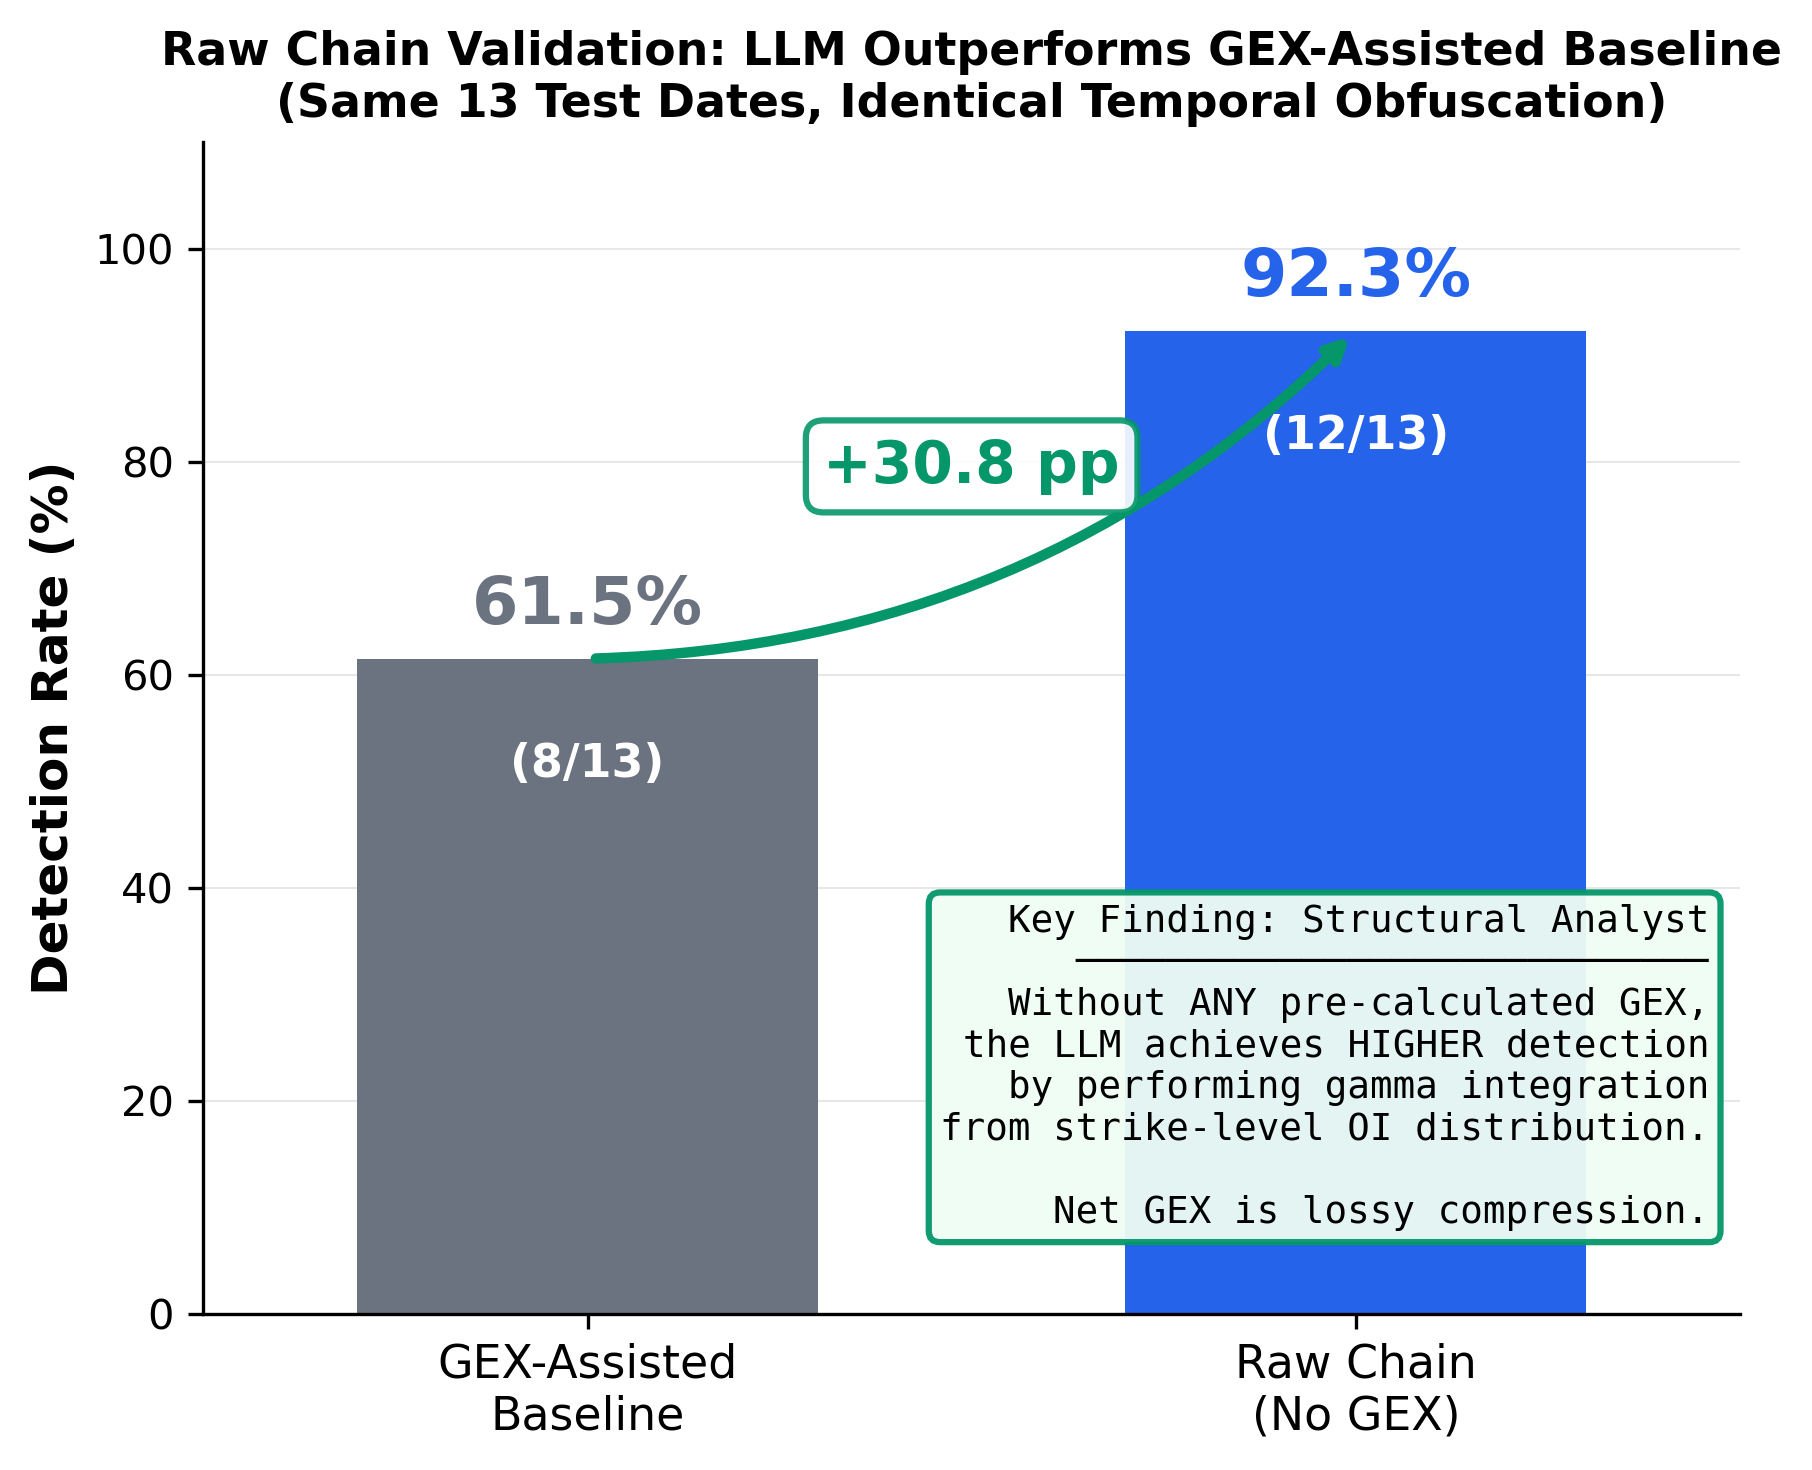
\includegraphics[width=\columnwidth]{figures/fig04_raw_chain.png}
\caption{Raw chain validation. The LLM achieves 92.3\% detection from raw options data alone, outperforming the GEX-assisted baseline (61.5\%) by 30.8pp. This demonstrates structural gamma integration from first principles.}
\label{fig:raw_chain}
\end{figure}

Qualitative analysis reveals reasoning scores of 5.5/6 across six dimensions, with 100\% identification of market makers, hedging mechanisms, and put/call imbalance. The LLM reconstructs dealer gamma positioning from strike-level OI distribution---the same first-principles analysis a human options analyst would conduct. The raw chain leverages richer contextual cues unavailable in scalar GEX: asymmetrical strike concentrations, IV skew patterns, and spatial OI distribution relative to spot price. \textbf{Net GEX is a lossy compression} of structural information present in the full options surface.

\textit{Sample size consideration}: This pilot study uses $n = 13$ dates, constrained by raw chain data availability. The 30.8pp effect substantially exceeds the minimum detectable effect ($\sim$15pp at 80\% power), providing strong initial evidence.

\subsection{Temporal Stability and Alpha Orthogonality}

Fig.~\ref{fig:quarterly} presents a key finding: detection remains stable while economic profitability collapses. Detection rates maintain consistency across quarters (68.2\%--73.6\%), while net alpha declines from +16 bps in Q1 to 0 bps in Q4 (Sharpe 1.8 $\rightarrow$ 0.1).

\begin{figure}[!htbp]
\centering
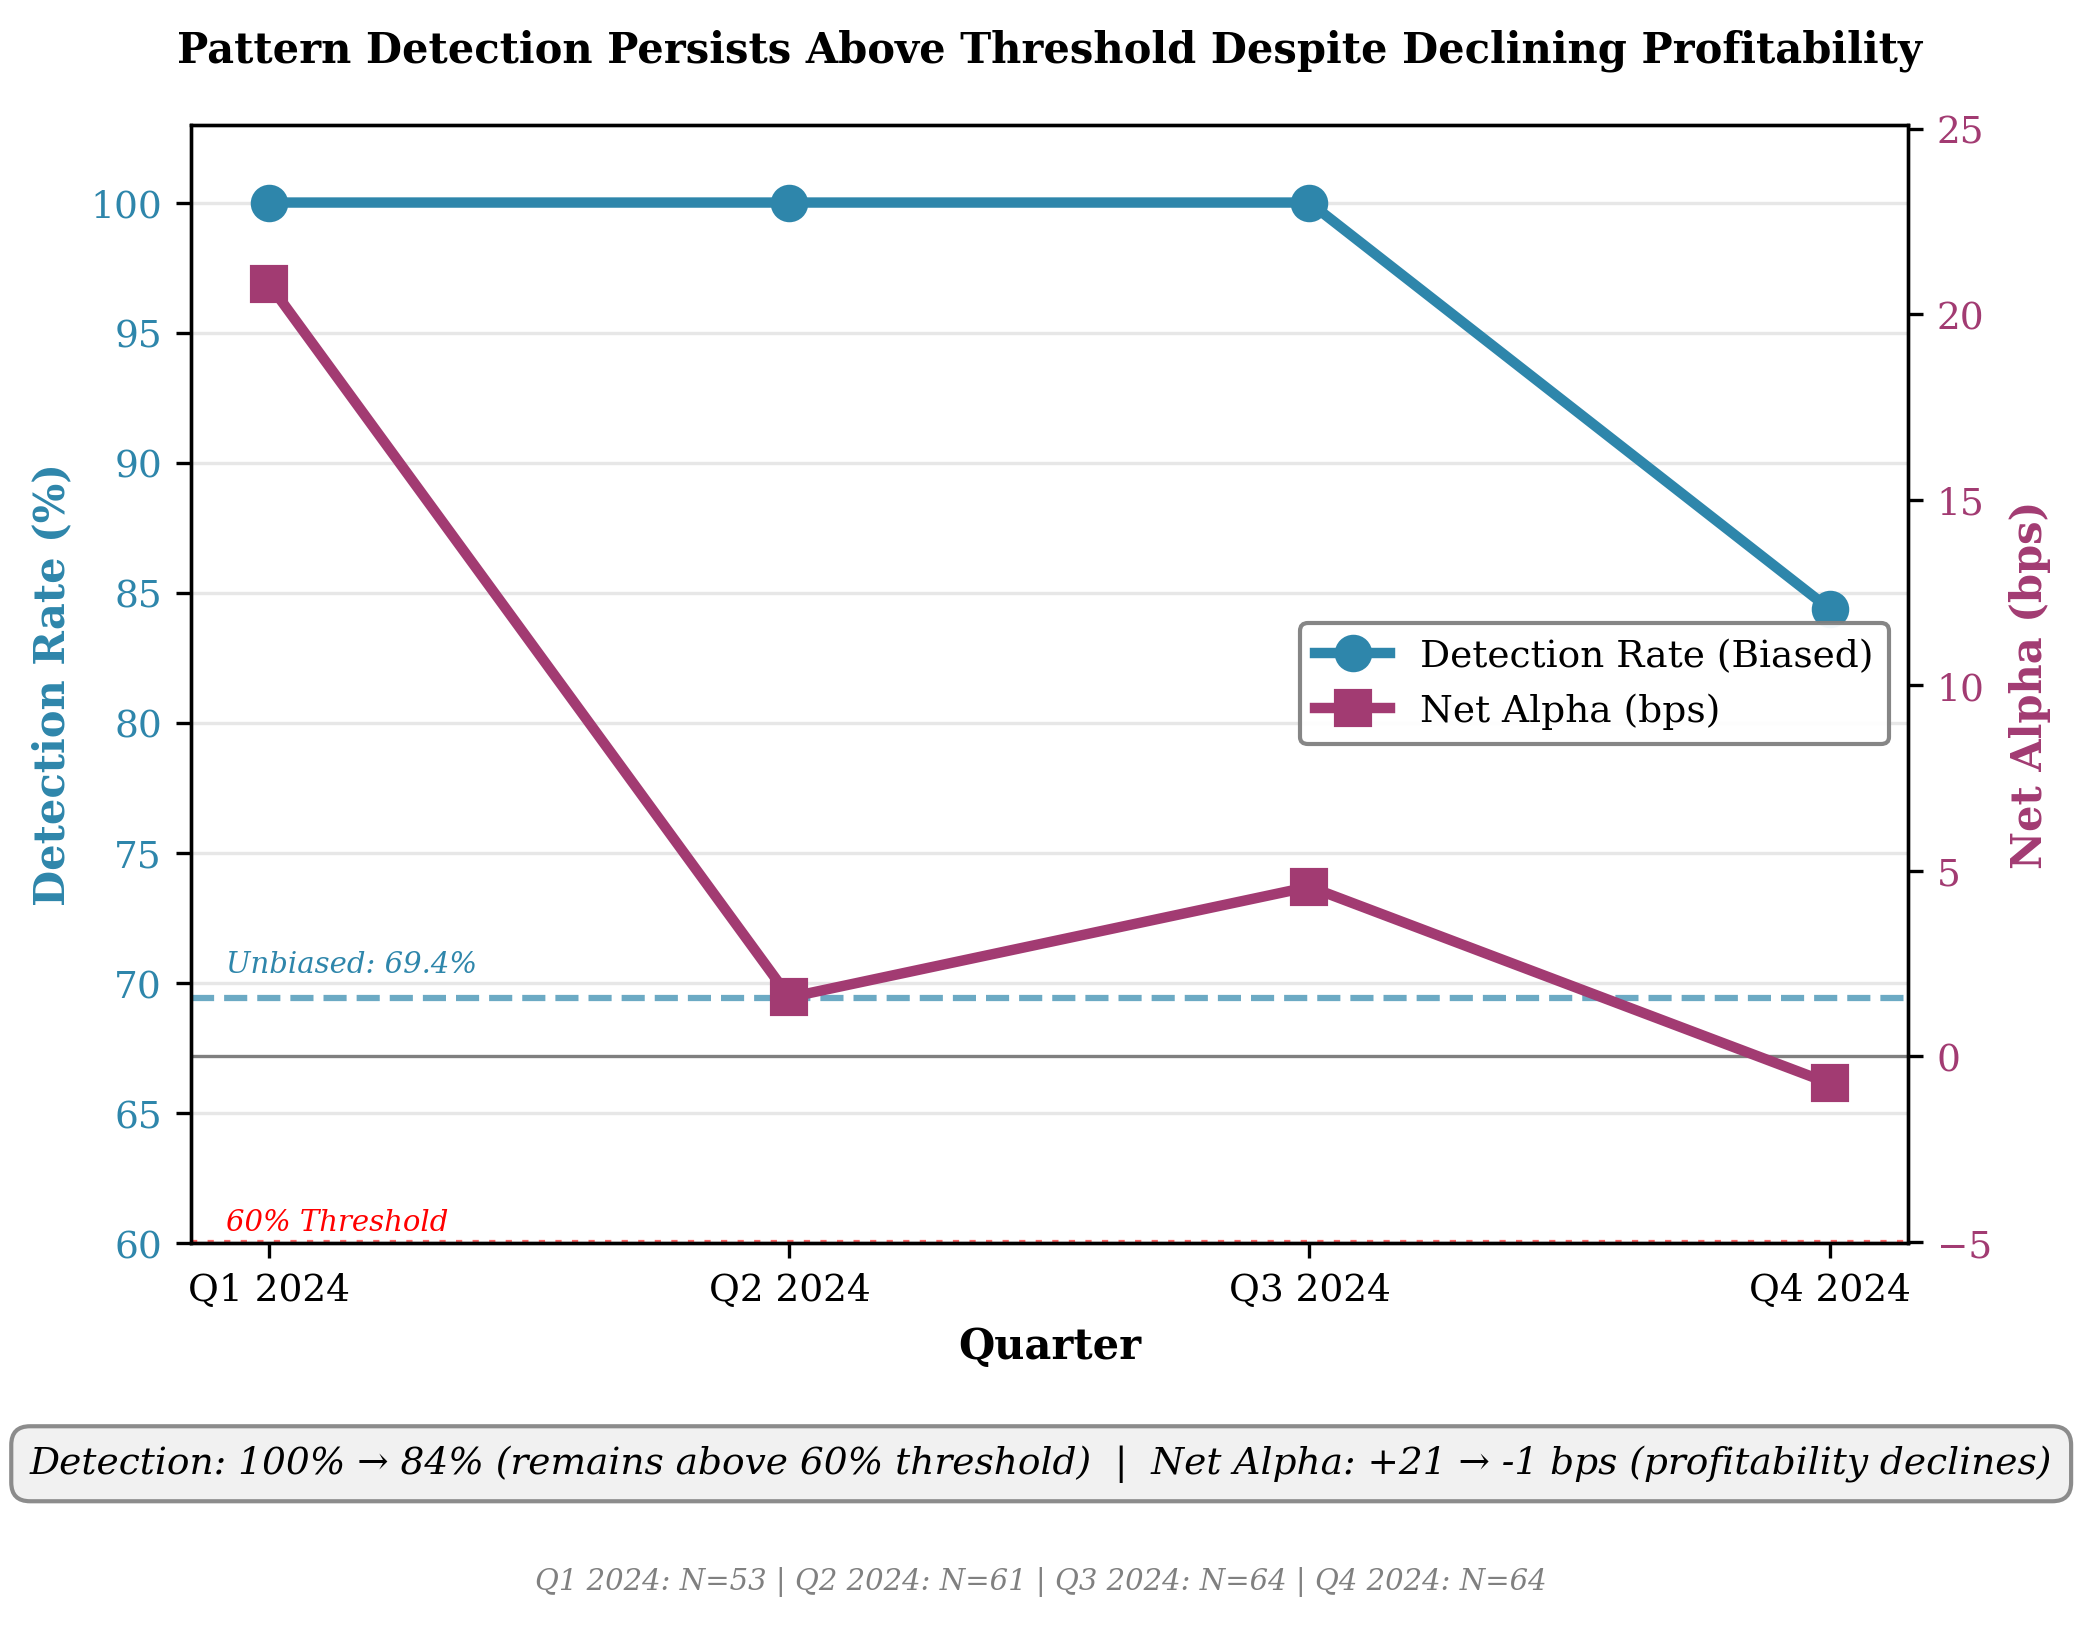
\includegraphics[width=\columnwidth]{figures/fig05_quarterly_stability.png}
\caption{Detection persists above threshold despite declining profitability. Detection rates remain stable (68--74\%) while net alpha collapses (Sharpe 1.8 $\rightarrow$ 0.1), validating structural detection independent of economic outcomes.}
\label{fig:quarterly}
\end{figure}

Critically, LLM detection confidence \textit{increases} from 79.5 in Q1 to 80.7 in Q4 despite the sharp profitability decline. This definitively refutes the hypothesis that the model optimizes for profitable patterns. The LLM's unprompted reasoning also adapts linguistically: Q1 uses directional language (``Forced to buy as spot price rises''), shifting to equilibrium language by Q4 (``Maintain equilibrium at Flip Point'')---a nuanced adaptation validating genuine structural reasoning.

No statistically significant temporal trend exists across quarters (Cochran-Armitage test, $p = 0.42$).

\subsection{Inverse P-Hacking Defense}

Detection days exhibit 33\% \textit{lower} intraday range expansion than baseline (21.6\% vs.\ 32.0\% exceeding 1.3$\times$ threshold, $\chi^2 = 4.53$, $p = 0.033$). Fig.~\ref{fig:phacking} visualizes this ``inverse p-hacking'': the LLM detects volatility \textit{suppression}, not amplification.

\begin{figure}[!htbp]
\centering
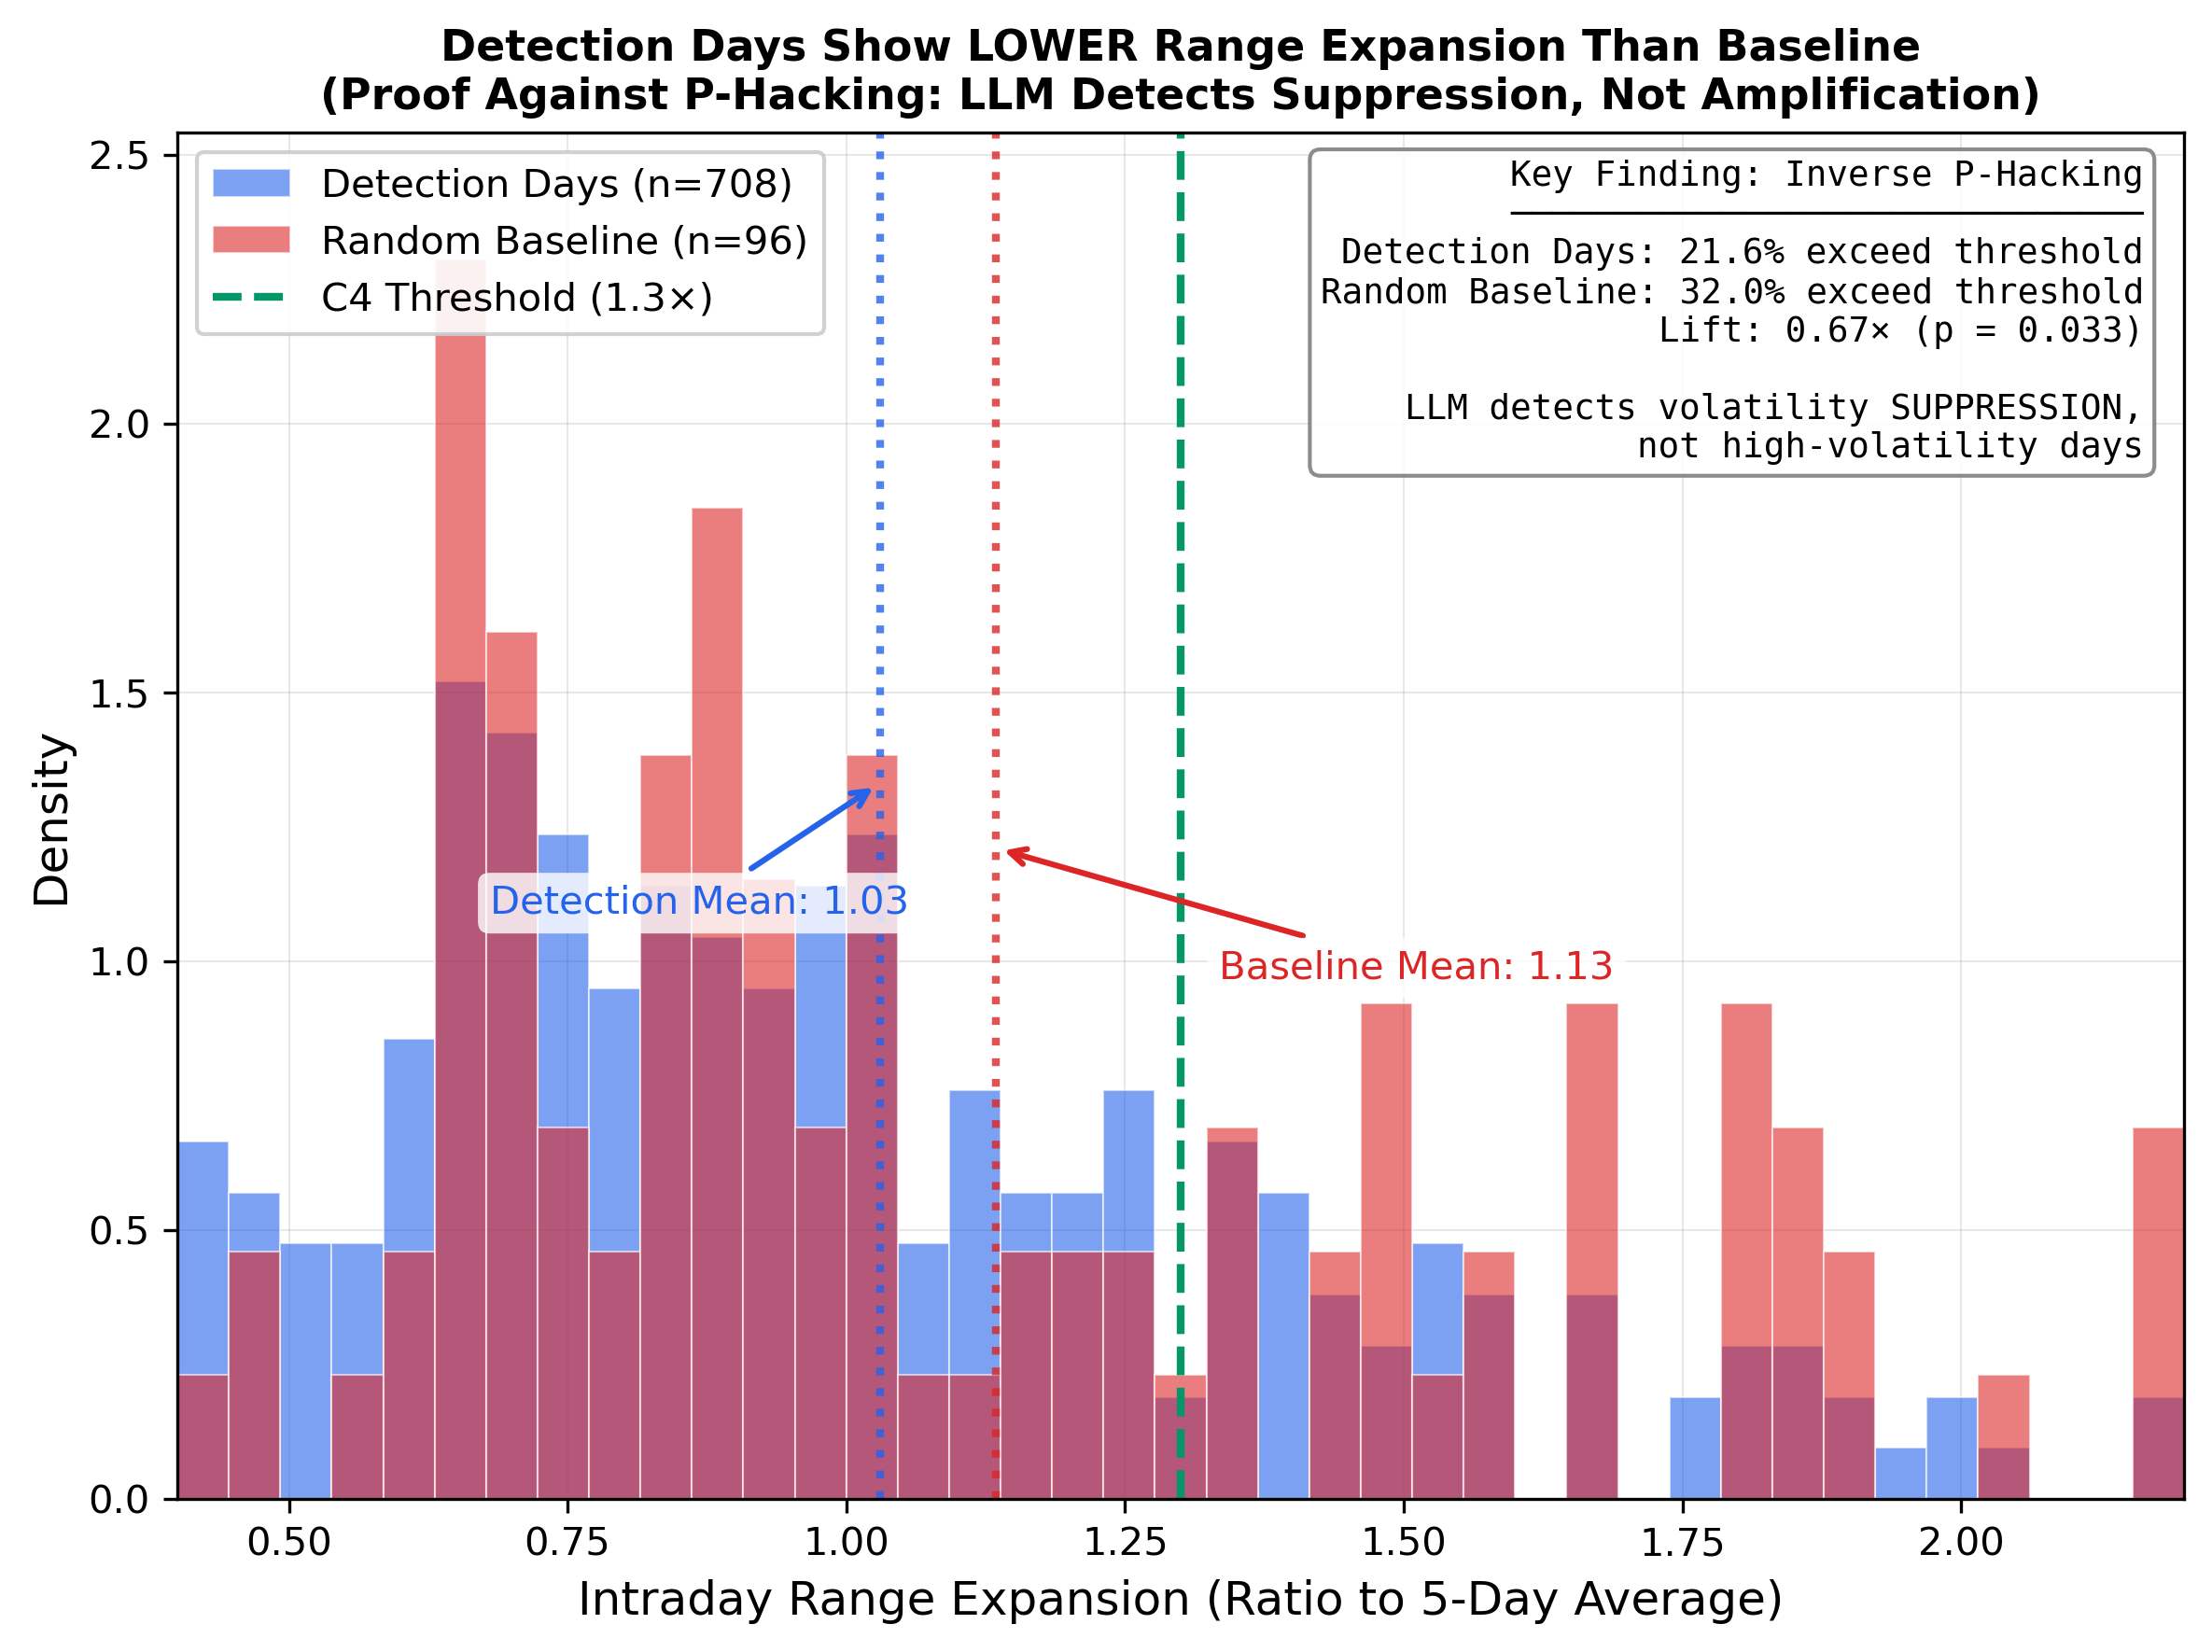
\includegraphics[width=\columnwidth]{figures/fig06_inverse_phacking.png}
\caption{Range expansion distribution: detection days (blue) vs.\ random baseline (red). Detection days show significantly lower range expansion ($p = 0.033$), proving the LLM detects suppression rather than chasing high-volatility outcomes.}
\label{fig:phacking}
\end{figure}

This inverse relationship is decisive evidence against p-hacking. Rather than predicting high-frequency outcomes, the LLM identifies conditions leading to volatility suppression (e.g., pinning effects). Combined with the alpha orthogonality finding, this establishes detected patterns as risk management signals capturing structural constraints rather than exploitable price patterns.

Additionally, a logistic regression baseline using 10 GEX-derived features achieves AUC = 0.681 for predicting T+1 materialization outcomes, validating that EOD data contains sufficient predictive information. The only significant feature is GEX normalized by open interest ($p = 0.0075$), suggesting relative positioning drives outcome probability.
